\documentclass[../../main.tex]{subfiles}

\begin{document}
\fexercisesHeader

\exercise{4.1}
\begin{wts}
    IF $\card{\xx}\geq 2$, there is a topology on $\xx$ that is $T_0$ but not $T_1$.
\end{wts}
\begin{proof}
    Let $\Tau_\xx = \{\varnothing\}\cup\{\{x\}\cup B,\: B\subseteq \xx\}$, where $x\in\xx$ is any point in $\xx$. Suppose $U_1$, and $U_2$ are open sets in $\Tau_\xx$, if either is empty then their intersection must be contained in $\Tau_\xx$. Otherwise $U_1 = \{x\}\cup B_1$, and $U_2 = \{x\}\cup B_2$, where $B_1$ and $B_2$ are subsets of $\xx$.
    \[
        U_1\cap U_2 = \{x\}(B_1\cap B_2)\in \Tau_\xx
    \]
    Notice also $\{\varnothing,\: \xx\}\subseteq\Tau_\xx$. Fix an arbitrary family of open sets $\{U_\alpha\}_{\alpha\in A}$, in similar fashion we have $\bigcup U_\alpha = \{x\}\cup\biggl( \bigcup B_{\alpha\in A} \biggr)$ so their union is contained in $\Tau_\xx$ as well.\\

    This topology is $T_0$. Fix $y\neq z$ in $\xx$, if either $y$ or $z$ is $x$, then choosing $\{x\}$ does the job. So assume $x\neq y\neq z\neq x$, and $\{y\}\cup \{x\}$ is an open set that does not contain $z$. This topology cannot be $T_1$, as $x$ sticks onto every open set, so there are no open sets which separate $x$ from the other points in $\xx$.
\end{proof}
\newpage

\exercise{4.2}
\begin{wts}
    If $\xx$ is an infinite set, the cofinite topology on $\xx$ is $T_1$ but not $T_2$, and is first countable iff $\xx$ is countable.
\end{wts}
\begin{proof}
    We will first verify that the cofinite topology $\Tau_\xx$ is a topology. 
    \[
        \Tau_\xx = \bigset{U,\quad U^c \text{ is finite.}}\cup \{\varnothing\}
    \]
    So that $\{\varnothing,\: \xx\}\subseteq\Tau_\xx$. Let $U_1$ and $U_2$ be a pair of open sets, assuming if neither of them are empty, then $U_2^c$ and $U_1^c$ are finite sets, so that $U_1^c\cup U_2^c$ is finite as well. Use DeMorgan to see that $U_1\cap U_2\in\Tau_\xx$.\\

    If $\{U_\alpha\}_{\alpha\in A}$ is an arbitrary collection of open sets, then 
    \[
        \bigcap_{\alpha\in A} U_\alpha^c\subseteq U_\beta^c
    \]
    where $\beta\in A$ is arbitrary, so $U_\beta^c$ is finite. And the union $\bigcup U_\alpha$ is contained in $\Tau_\xx$.\\

    To show that $\Tau_\xx$ is $T_1$, every singleton set is closed. To show that $\Tau_\xx$ is not $T_2$, fix $x\neq y$. If $B_x$ and $B_y$ are open sets that contain $x$ and $y$ respectively. If $B_x$ and $B_y$ disjoint, then 
    \[
        B_x\subseteq B_y^c
    \]
    Which means $B_x$ is an open, finite subset. But the only open and finite subset of $\xx$ is the empty set. This contradicts $x\in B_x$.\\

    If $\xx$ is countable, we will find a neighbourhood base $\nb{x}$ for any $x \in \xx$ as follows: 
    \begin{itemize}
        \item We can index $\xx$ using $\nat^+\cup\{0\}$, so without loss of generality, let $x_0 = x$, and 
        \item Define $U_1 = \{x_1\}^c$, and $U_n = \bigcap_{j=1}^n \{x_j\}^c$ are open sets that contain $x$. Equivalently,
        \[
            U_n = \bigset{x_j,\: j\geq n+1}\cup\{x_0\}
        \]
        \item If $V$ is an open set that contains $x_0$, then $V^c$ is finite, let $M\in\nat^+$ be the largest index of $x_j\notin V$ (the negation of this is that if $j\geq M+1$, then $x_j\in V$) then $U_{M+1}\subseteq V$ as needed, and $\xx$ is first countable.
    \end{itemize}
    Conversely, if $\xx$ is first countable, we can find a descending sequence of neighbourhoods which form a neighbourhood base, $\{U_j\}_{j\geq 1}\subseteq \Tau_\xx$. And each $U_j^c$ is finite, so $\bigcup U_j^c$ is countable. Assume for contradiction that $\xx$ is uncountable, then 
    \[
        \bigcup U_j^c = \biggl(\bigcap U_j\biggr)^c
    \]
    is countable, hence the intersection $\bigcap U_j$ must be uncountable (hence infinite). Pick $y\neq x$, where $y$ belongs in the intersection of all neighbourhoods $U_j$. This contradicts the fact that $\{U_j\}$ is a neighbourhood base, as $x$ is an element in the open set $\{y\}^c$ therefore there must be a $U_k$ 
    \[
        x\in U_k\subseteq \{y\}^c
    \]
    But $y\in U_k$ for each $U_k$ and the proof is complete.
\end{proof}
\newpage

\exercise{4.3}
\begin{wts}
    Every metric space is normal. (If $A,B$ are disjoint closed sets in the metric space, consider the set of points $x$ where $d(x,A)< d(x,B)$ or $d(x,A)> d(x,B)$).
\end{wts}
\begin{proof}
    First, we show that if $A$ is closed, then $d(x,A) = 0\iff x\in A$. If $x\in A$, then $d(x,A)\leq d(x,x) = 0$. if $x\notin A$, then there exists a ball of radius $\varepsilon>0$ where $B(\varepsilon, x)\cap A = \varnothing$. Hence, $\varepsilon$ is a lower bound for the set $\{d(x,y),\: y\in A\}$, taking the infimum over this set we see that $d(x,A)\geq \varepsilon>0$.\\

    Fix some $x\in \Phi_A$ where $\Phi_A = \bigset{y\in\xx, d(y,A) < d(y,B)}$. We wish to find an open ball about $x$ that is contained in $\Phi_A$. The Triangle Inequality works for this definition of distance as well, as
    \begin{equation}\label{eq:function-infimum}
        f(a)\leq g(a), \forall a\in A\implies \inf_{a\in A}f(a)\leq \inf_{a\in A}g(a)
    \end{equation}
    If $a\in A$, then $d(z,A)\leq d(x,z) + d(x,A)$, using \Cref{eq:function-infimum} yields 
    \[
        \begin{cases}
            d(z,A)\leq d(x,A) + d(x,z)\\
            d(x,B)-d(x,z)\leq d(z,B)
        \end{cases}
    \]
    where $z\in B(\varepsilon, x)$ so $d(x,z)\lsim\varepsilon$. The second estimate above is found by 'flipping an upper bound to become a lower bound'. We can choose $d(x,z)$ sufficiently small that 
    \[
        d(x,A) + d(x,z) < d(x,B) - d(x,z)
    \]
    in order to 'pipe' the two inequalities, so
    \begin{equation}\label{ex:4.3-distance-estimate}
        2d(x,z) < d(x,B) - d(x,A)
    \end{equation}
    Take $\varepsilon = [d(x,B) - d(x,A)]3^{-1}$, then $z\in B(\varepsilon, x)$ implies $d(x,z)<\varepsilon$, and \Cref{ex:4.3-distance-estimate} holds. See \Cref{fig:ex4.3} for details.\\
\begin{figure}
    \centering
    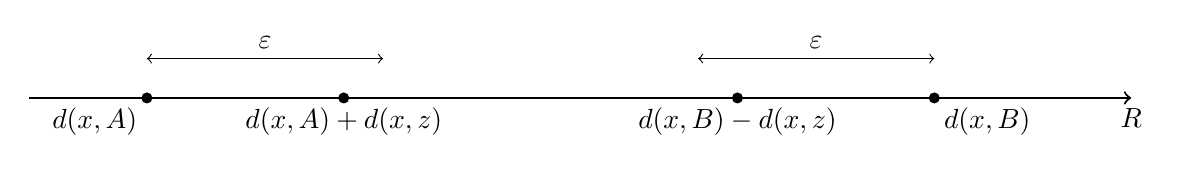
\begin{tikzpicture}
    % Draw the real line
    \draw[thick,->] (-0.5,0) -- (13.5,0) node[below] {$\mathbb{R}$};
    
    % Left Markers
    \fill (1,0) circle (2pt);
    \fill (3.5,0) circle (2pt);
    \node[below left] at (1,0) {$d(x,A)$};
    \node[below] at (3.5,0) {$d(x,A) + d(x,z)$};
    \draw[<->] (1,0.5) -- (4,0.5) node[midway,above] {$\varepsilon$};

    % Right MRakers
    \fill (8.5,0) circle (2pt);
    \fill (11,0) circle (2pt);
    \node[below right] at (11,0) {$d(x,B)$};
    \node[below] at (8.5,0) {$d(x,B) - d(x,z)$};
    \draw[<->] (8,0.5) -- (11,0.5) node[midway,above] {$\varepsilon$};
    
    
\end{tikzpicture}
    \caption{Exercise 4.3: Finding a $\varepsilon$ small enough that fits within $d(x,A) < d(x,B)$}
    \label{fig:ex4.3}
\end{figure}
\end{proof}
\newpage

\exercise{4.4}
\begin{wts}
    
\end{wts}
\begin{proof}
    
\end{proof}

\exercise{4.16}
\begin{wts}
\end{wts}

\begin{proof}
    \begin{enumalpha}
        \item[]
        \item Let $x\in \{f\neq g\}$, then there exists disjoint open subsets of $\yy$, $f(x)\in U$ and $g(x)\in V$, $U\cap V=\varnothing$, but $f^{-1}(U)\cap g^{-1}(V)$ is an open set in $\xx$ that contains $x$. Therefore $\{f\neq g\}$ is open in $\xx$.
        \item Suppose $\{f=g\}=E$ is dense in $\xx$. Let $x\in E$, induces two disjoint open sets exactly like in part a. This is an open set that contains $x$, and $y\in f^{-1}(U)\cap g^{-1}(V)\cap E$. Since $y\in E$, it follows that $f(y) = g(y)$, and
        \[
            \begin{cases}
            y\in f^{-1}(U)\implies &f(y)\in U\\
            y\in g^{-1}(V)\implies &g(y)\in V
            \end{cases}
        \]
    \end{enumalpha}
\end{proof}
\newpage


\exercise{4.17}



\end{document}